\begin{figure} \centering 
\begin{minipage}{.35\textwidth}
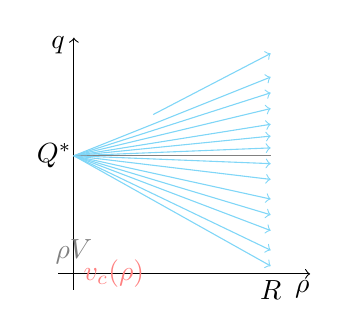
\begin{tikzpicture}

% coordinates
\draw[->] (0,-0.2) -- (0,3);
\draw[->] (-0.2,0) -- (3,0);
% rarefactions
\draw[->][cyan!50] (0, 1.5) -- (2.5, 1.6) ;
\draw[->][cyan!50] (0, 1.5) -- (2.5, 1.75) ;
\draw[->][cyan!50] (0, 1.5) -- (2.5, 1.9) ;
\draw[->][cyan!50] (0, 1.5) -- (2.5, 2.1) ;
\draw[->][cyan!50] (0, 1.5) -- (2.5, 2.3) ;
\draw[->][cyan!50] (0, 1.5) -- (2.5, 2.5) ;
\draw[->][cyan!50] (1.008, 2.024) -- (2.5, 2.8) ;cri

\draw[black!50] (0, 1.5) -- (1.5, 1.5) ;
\draw[black!50] (1.5, 1.5) -- (2.5, 1.5) ;

\draw[->][cyan!50] (0, 1.5) -- (2.5, 1.4) ;
\draw[->][cyan!50] (0, 1.5) -- (2.5, 1.2) ;
\draw[->][cyan!50] (0, 1.5) -- (2.5, 0.95) ;
\draw[->][cyan!50] (0, 1.5) -- (2.5, 0.75) ;
\draw[->][cyan!50] (0, 1.5) -- (2.5, 0.55) ;
\draw[->][cyan!50] (0, 1.5) -- (2.5, 0.3) ;
\draw[->][cyan!50] (0, 1.5) -- (2.5, 0.1) ;

\draw[black!50, domain=0:0.4] plot[id=x] function{7*x} node[above] {$\rho V$};
\draw[orange!50, domain=0:0.85]  plot[id=x] function{x*(x+2.5)};
\draw[red!50, domain=0:1.25]  plot[id=x] function{x*(x+1)}  node[right] {$v_c(\rho)$};

\node at (2.5, -0.2) {$R$};
\node at (-0.25, 1.5) {$Q^{*}$};
\node at (2.9, -0.2) {$\rho$};
\node at (-0.2, 2.9) {$q$};

\end{tikzpicture}
\caption{The fundamental diagram}
\label{Fig:}
\end{minipage}
\begin{minipage}{.35\textwidth}
\begin{tikzpicture}
\draw[->] (0,-0.2) -- (0,2);
\draw[->] (-0.2,0) -- (2.5,0);
\draw[cyan!50]  plot [smooth, tension = 1.5] coordinates { (0,0) (1,1) (2,0)};
\node at (2, -0.2) {$R$};
%\node at (-0.2, 2) {$V$};
\node at (2.6, -0.2) {$\rho $};
\node at (-0.2, 2.1) {$\rho v$};
\end{tikzpicture}
\caption{}
\label{Fig:}
\end{minipage}
\end{figure}